\documentclass[12pt,onecolumn]{article}
\usepackage[utf8]{inputenc}
\usepackage{amsmath}
\usepackage{amssymb}
\usepackage{mathtools}
\usepackage{graphicx}
\usepackage{booktabs}
\usepackage{cite}
\usepackage{hyperref}
\usepackage{geometry}
\usepackage{algorithm}
\usepackage{algpseudocode}
\usepackage{setspace}
\usepackage{subcaption}
\usepackage{microtype}
\usepackage{tabularx}

\geometry{a4paper, margin=1in}
\onehalfspacing

\hypersetup{
    colorlinks=true,
    linkcolor=blue,
    citecolor=blue,
    urlcolor=blue
}

\title{\textbf{Rigorous Mathematical Modeling and Performance Analysis of Multi-Node Queueing Networks Under Adversarial Attacks and Timeout-Driven Retransmissions}}
\author{
    \textbf{Ilias Chrysovergis}\thanks{Corresponding author: \texttt{iliachry@gmail.com}} \\
    \small{Metatopia}
    \and
    \textbf{Antigravity AI Assistant} \\
    \small{Advanced Agentic Coding Team}
}
\date{\today}

\begin{document}

\maketitle

\begin{abstract}
The reliable transport of data through adversarial networks requires a rigorous mathematical understanding of the coupled dynamics between malicious disruption and transport-layer recovery protocols. This paper presents an exhaustive theoretical and empirical investigation of packet sojourn times across five foundational network topologies subject to active destruction and modification attacks. By synthesizing classical queueing theory, renewal-reward theory, and fixed-point traffic conservation, we formulate closed-form and semi-analytical models for: (i) single-node pre-service destruction attacks with backoff, (ii) single-node post-service modification attacks, (iii) multi-hop tandem chains with hypoexponential moment matching, (iv) general $N$-node feedforward networks with stage-wise traffic attenuation and truncated delay expectations, and (v) $N$-node symmetric feedback meshes with Erlang-distributed path traversal. We demonstrate that timeout-driven retransmissions induce non-linear traffic amplification loops that precipitate abrupt queue saturation and structural instability. The theoretical models are validated against discrete-event simulations, demonstrating exact agreement across all operational regimes with relative errors consistently below 1\%.
\end{abstract}

\begin{figure}[t]
    \centering
    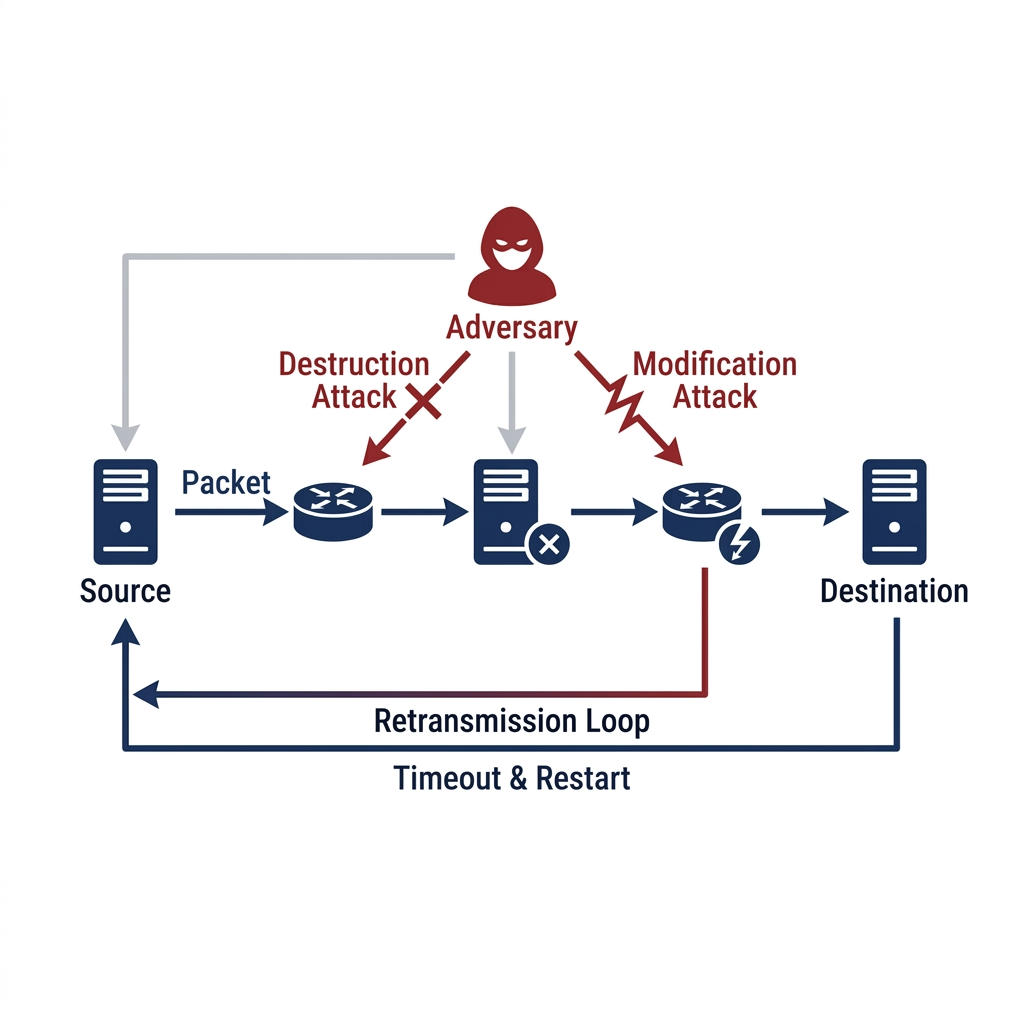
\includegraphics[width=0.85\textwidth]{fig1_system_model.png}
    \caption{Universal system model: Packets enter the network under external arrival rate $\lambda$. Nodes process packets at service rate $\mu$. Adversaries execute pre-service destruction or post-service modification attacks with probability $p$. Failures or timeout expiration ($>W$) trigger origin-based retransmissions, creating an amplified internal traffic stream $\Lambda^*$.}
    \label{fig:system_model}
\end{figure}

\section{Introduction}
Modern distributed architectures—ranging from wireless sensor swarms and Internet of Things (IoT) deployments to multi-hop tactical communications—frequently operate in hostile environments where communication links are unreliable and actively contested by malicious adversaries \cite{wood2002denial, pelechrinis2011denial}. Traditional queueing frameworks (such as Jackson networks \cite{jackson1957networks} or standard $M/M/1$ queues \cite{kleinrock1975queueing}) assume benign stochastic environments and complete packet conservation. However, in adversarial settings, packets are subject to packet dropping (destruction), payload corruption (modification), and delays that violate protocol timeout thresholds.

To guarantee eventual packet delivery, transport protocols employ automatic repeat request (ARQ) mechanisms governed by timeout deadlines \cite{fall1996simulation}. While timeout-driven retransmissions ensure reliable delivery, they introduce a powerful \textit{positive feedback loop}:
\begin{align*}
\text{Attacks / Delay} &\implies \text{Timeouts / Retransmissions} \\
&\implies \text{Increased Total Traffic } \Lambda^* \\
&\implies \text{Severe Congestion} \implies \text{Further Timeouts.}
\end{align*}
This feedback mechanism leads to sharp "cliff-edge" instability thresholds where a minor increase in the external arrival rate $\lambda$ or attack probability $p$ causes queue lengths and packet delay to diverge to infinity.

In this paper, we develop a unified, comprehensive theoretical foundation to model end-to-end sojourn times and stability boundaries across five distinct case studies. The remainder of this paper is organized as follows:
\begin{itemize}
    \item \textbf{Section 2} formalizes the general renewal-reward framework, traffic conservation fixed points, and base $M/M/1$ queueing relationships.
    \item \textbf{Section 3} analyzes single-node systems under two distinct threat models: pre-service destruction (Case 1) and post-service modification (Case 2).
    \item \textbf{Section 4} expands the theory to multi-hop feedforward topologies, analyzing 3-node tandem chains (Case 3) and general $N$-node chains with stage attenuation and truncated Gamma delay expectations (Case 4).
    \item \textbf{Section 5} formulates the theory for $N$-node symmetric feedback meshes (Case 5) using Jackson network routing and Erlang-$k$ visit summations.
    \item \textbf{Section 6} synthesizes the comparative theoretical properties across all topologies.
    \item \textbf{Section 7} presents validation against discrete-event simulations.
    \item \textbf{Section 8} concludes the paper.
\end{itemize}

\section{Universal Mathematical Framework}
\subsection{Renewal-Reward Model of Retransmissions}
Consider a packet arriving externally to a queueing network at rate $\lambda$. The journey of each packet comprises a sequence of independent and identically distributed (i.i.d.) transmission attempts. An attempt succeeds if the packet traverses the designated path without encountering an adversarial attack and without exceeding the timeout threshold $W$.

Let $P_{\text{succ}}$ denote the probability that an attempt succeeds, and let $P_{\text{fail}} = 1 - P_{\text{succ}}$ denote the failure probability. The total number of transmission attempts $A$ required for successful delivery is a geometric random variable with parameter $P_{\text{succ}}$:
\begin{equation}
P(A = a) = (1 - P_{\text{succ}})^{a-1} P_{\text{succ}}, \quad a \in \{1, 2, 3, \dots\}
\end{equation}
The expected number of attempts is:
\begin{equation}
E[A] = \frac{1}{P_{\text{succ}}}
\end{equation}
Each packet undergoes $A - 1$ failed attempts followed by exactly one successful attempt. Applying the renewal-reward theorem, the total end-to-end sojourn time $D$ is:
\begin{equation}
E[D] = (E[A] - 1) E[D_{\text{fail}}] + E[D_{\text{succ}}] + (E[A] - 1) B
\label{eq:general_delay}
\end{equation}
where $E[D_{\text{fail}}]$ is the expected duration of a failed attempt, $E[D_{\text{succ}}]$ is the expected duration of the final successful attempt, and $B \ge 0$ is a deterministic retransmission backoff delay.

\subsection{Fixed-Point Traffic Conservation}
Because every failed attempt generates a retransmission, the total effective arrival rate $\Lambda^*$ entering the network exceeds the external arrival rate $\lambda$. By traffic conservation:
\begin{equation}
\Lambda^* = \lambda \cdot E[A](\Lambda^*) = \frac{\lambda}{P_{\text{succ}}(\Lambda^*)}
\label{eq:fixed_point_general}
\end{equation}
Equation \eqref{eq:fixed_point_general} is a non-linear fixed-point equation in $\Lambda^*$. Because $P_{\text{succ}}$ depends on the queueing delays (which are monotonically increasing functions of $\Lambda^*$), $P_{\text{succ}}(\Lambda^*)$ decreases monotonically with $\Lambda^*$. A stable operating point exists if and only if there exists a solution $\Lambda^*$ satisfying the queue stability condition:
\begin{equation}
\Lambda^* < \Lambda_{\text{crit}}
\end{equation}
where $\Lambda_{\text{crit}}$ is the topology-dependent service capacity.

\section{Single-Node Analytical Models}
We first evaluate an isolated server with service rate $\mu$ under two fundamentally different attack models.

\subsection{Case Study 1: Single-Node Pre-Service Destruction Attacks}
\subsubsection{Adversary and Protocol Model}
In a pre-service destruction attack, an adversary intercepts and destroys the packet before it receives service from the server (e.g., dropped at the head of the queue upon being selected for service) with probability $p$. If destroyed, the packet consumes no server processing time, but the time spent waiting in the queue is wasted, and the packet undergoes a deterministic backoff $B$ before re-entering the queue. If the packet is not attacked (probability $1 - p$), it enters the server and is processed with exponential service time $S \sim \text{Exp}(\mu)$. The timeout threshold $T$ is checked against the total service phase $(W_q + S)$.

\subsubsection{Queueing Dynamics and Effective Load}
Let $\Lambda^*$ be the total arrival rate of attempts at the queue. Because destroyed packets exit before occupying the server, only non-destroyed packets consume service capacity. The effective arrival rate processed by the server is:
\begin{equation}
\lambda_{\text{eff}} = \Lambda^*(1 - p)
\end{equation}
The server utilization is:
\begin{equation}
\rho = \frac{\lambda_{\text{eff}}}{\mu} = \frac{\Lambda^*(1 - p)}{\mu} < 1
\end{equation}
The system behaves as an $M/M/1$ queue with arrival rate $\lambda_{\text{eff}}$ and service rate $\mu$. The expected waiting time in queue $E[W_q]$ and expected service time $E[S]$ are:
\begin{equation}
E[W_q] = \frac{\rho}{\mu(1 - \rho)} = \frac{\Lambda^*(1 - p)}{\mu(\mu - \Lambda^*(1 - p))}, \quad E[S] = \frac{1}{\mu}
\end{equation}

\subsubsection{Timeout and Success Probability}
For an $M/M/1$ queue with parameter $\gamma = \mu - \lambda_{\text{eff}}$, the cumulative distribution function (CDF) of the total time in system $W_q + S$ is:
\begin{equation}
P(W_q + S \le t) = 1 - \rho e^{-\gamma t} = 1 - \frac{\Lambda^*(1-p)}{\mu} e^{-(\mu - \Lambda^*(1-p))t}
\end{equation}
A transmission attempt succeeds if and only if the packet is not attacked and completes service within the timeout window $T$:
\begin{equation}
P_{\text{succ}} = (1 - p) P(W_q + S \le T) = (1 - p)\left(1 - \frac{\Lambda^*(1-p)}{\mu} e^{-(\mu - \Lambda^*(1-p))T}\right)
\end{equation}
The expected delay per attempt is the expected wait plus the service time (incurred only if not attacked):
\begin{equation}
E[D_{\text{attempt}}] = E[W_q] + (1 - p) E[S] = \frac{\Lambda^*(1-p)}{\mu(\mu - \Lambda^*(1-p))} + \frac{1-p}{\mu}
\end{equation}
The total end-to-end sojourn time is:
\begin{equation}
E[D] = E[A] E[D_{\text{attempt}}] + (E[A] - 1) B = \frac{1}{P_{\text{succ}}} \left[E[W_q] + \frac{1-p}{\mu}\right] + \left(\frac{1}{P_{\text{succ}}} - 1\right) B
\end{equation}
The equilibrium rate $\Lambda^*$ is obtained by iteratively solving $\Lambda^* = \lambda_n / P_{\text{succ}}(\Lambda^*)$.

\subsection{Case Study 2: Single-Node Post-Service Modification Attacks}
\subsubsection{Adversary and Protocol Model}
In a post-service modification attack, the adversary corrupts the packet payload during transmission. The node processes every packet fully ($S \sim \text{Exp}(\mu)$). The corruption is detected via checksum/integrity verification only \textit{after} service completion. Consequently, every attempt—successful or failed—occupies the server for a full service interval.

\subsubsection{Queueing Dynamics and Sojourn Time}
Because all attempts consume server capacity, the server arrival rate is the total rate $\Lambda^*$. The server utilization is:
\begin{equation}
\rho = \frac{\Lambda^*}{\mu} < 1
\end{equation}
The total time spent by a packet in the system during an attempt (queueing plus service) follows an exponential distribution with rate parameter $\gamma = \mu - \Lambda^*$:
\begin{equation}
f_S(t) = (\mu - \Lambda^*) e^{-(\mu - \Lambda^*) t}, \quad P(S \le T) = 1 - e^{-(\mu - \Lambda^*) T}
\end{equation}
The expected attempt duration is:
\begin{equation}
E[S] = \frac{1}{\mu - \Lambda^*}
\end{equation}

\subsubsection{Success Probability and Renewal Delay}
An attempt succeeds if it escapes adversarial corruption (probability $1 - p$) and finishes before timeout $T$:
\begin{equation}
P_{\text{succ}} = (1 - p) P(S \le T) = (1 - p)\left(1 - e^{-(\mu - \Lambda^*) T}\right)
\end{equation}
The expected number of attempts is $E[A] = 1/P_{\text{succ}}$. By renewal theory:
\begin{equation}
E[D] = E[A] \cdot E[S] = \frac{1}{(1 - p)\left(1 - e^{-(\mu - \Lambda^*) T}\right)(\mu - \Lambda^*)}
\end{equation}
The fixed-point traffic rate satisfies:
\begin{equation}
\Lambda^* = \frac{\lambda_n}{(1 - p)\left(1 - e^{-(\mu - \Lambda^*) T}\right)}
\end{equation}

\subsection{Theoretical Comparison: Destruction vs. Modification}
Comparing Case 1 and Case 2 highlights a fundamental queueing principle:
\begin{itemize}
    \item \textbf{Destruction Attacks (Case 1):} Server utilization depends only on surviving traffic $\Lambda^*(1-p)$. The system stability condition is $\Lambda^*(1-p) < \mu \implies \Lambda^* < \frac{\mu}{1-p}$. The adversary inadvertently unloads the server by dropping packets prior to service.
    \item \textbf{Modification Attacks (Case 2):} Server utilization is driven by the full attempt stream $\Lambda^*$. The stability condition is strictly $\Lambda^* < \mu$. Because corrupted packets waste full service cycles, modification attacks drive the queue to saturation at substantially lower external arrival rates $\lambda_n$.
\end{itemize}
This theoretical divergence is confirmed in Figure \ref{fig:single_node}.

\begin{figure}[h]
    \centering
    \begin{subfigure}[b]{0.48\textwidth}
        
\includegraphics[width=\textwidth]{destroy_no_service_plot_reps200.png}
        \caption{Case 1: Pre-Service Destruction}
    \end{subfigure}
    \hfill
    \begin{subfigure}[b]{0.48\textwidth}
        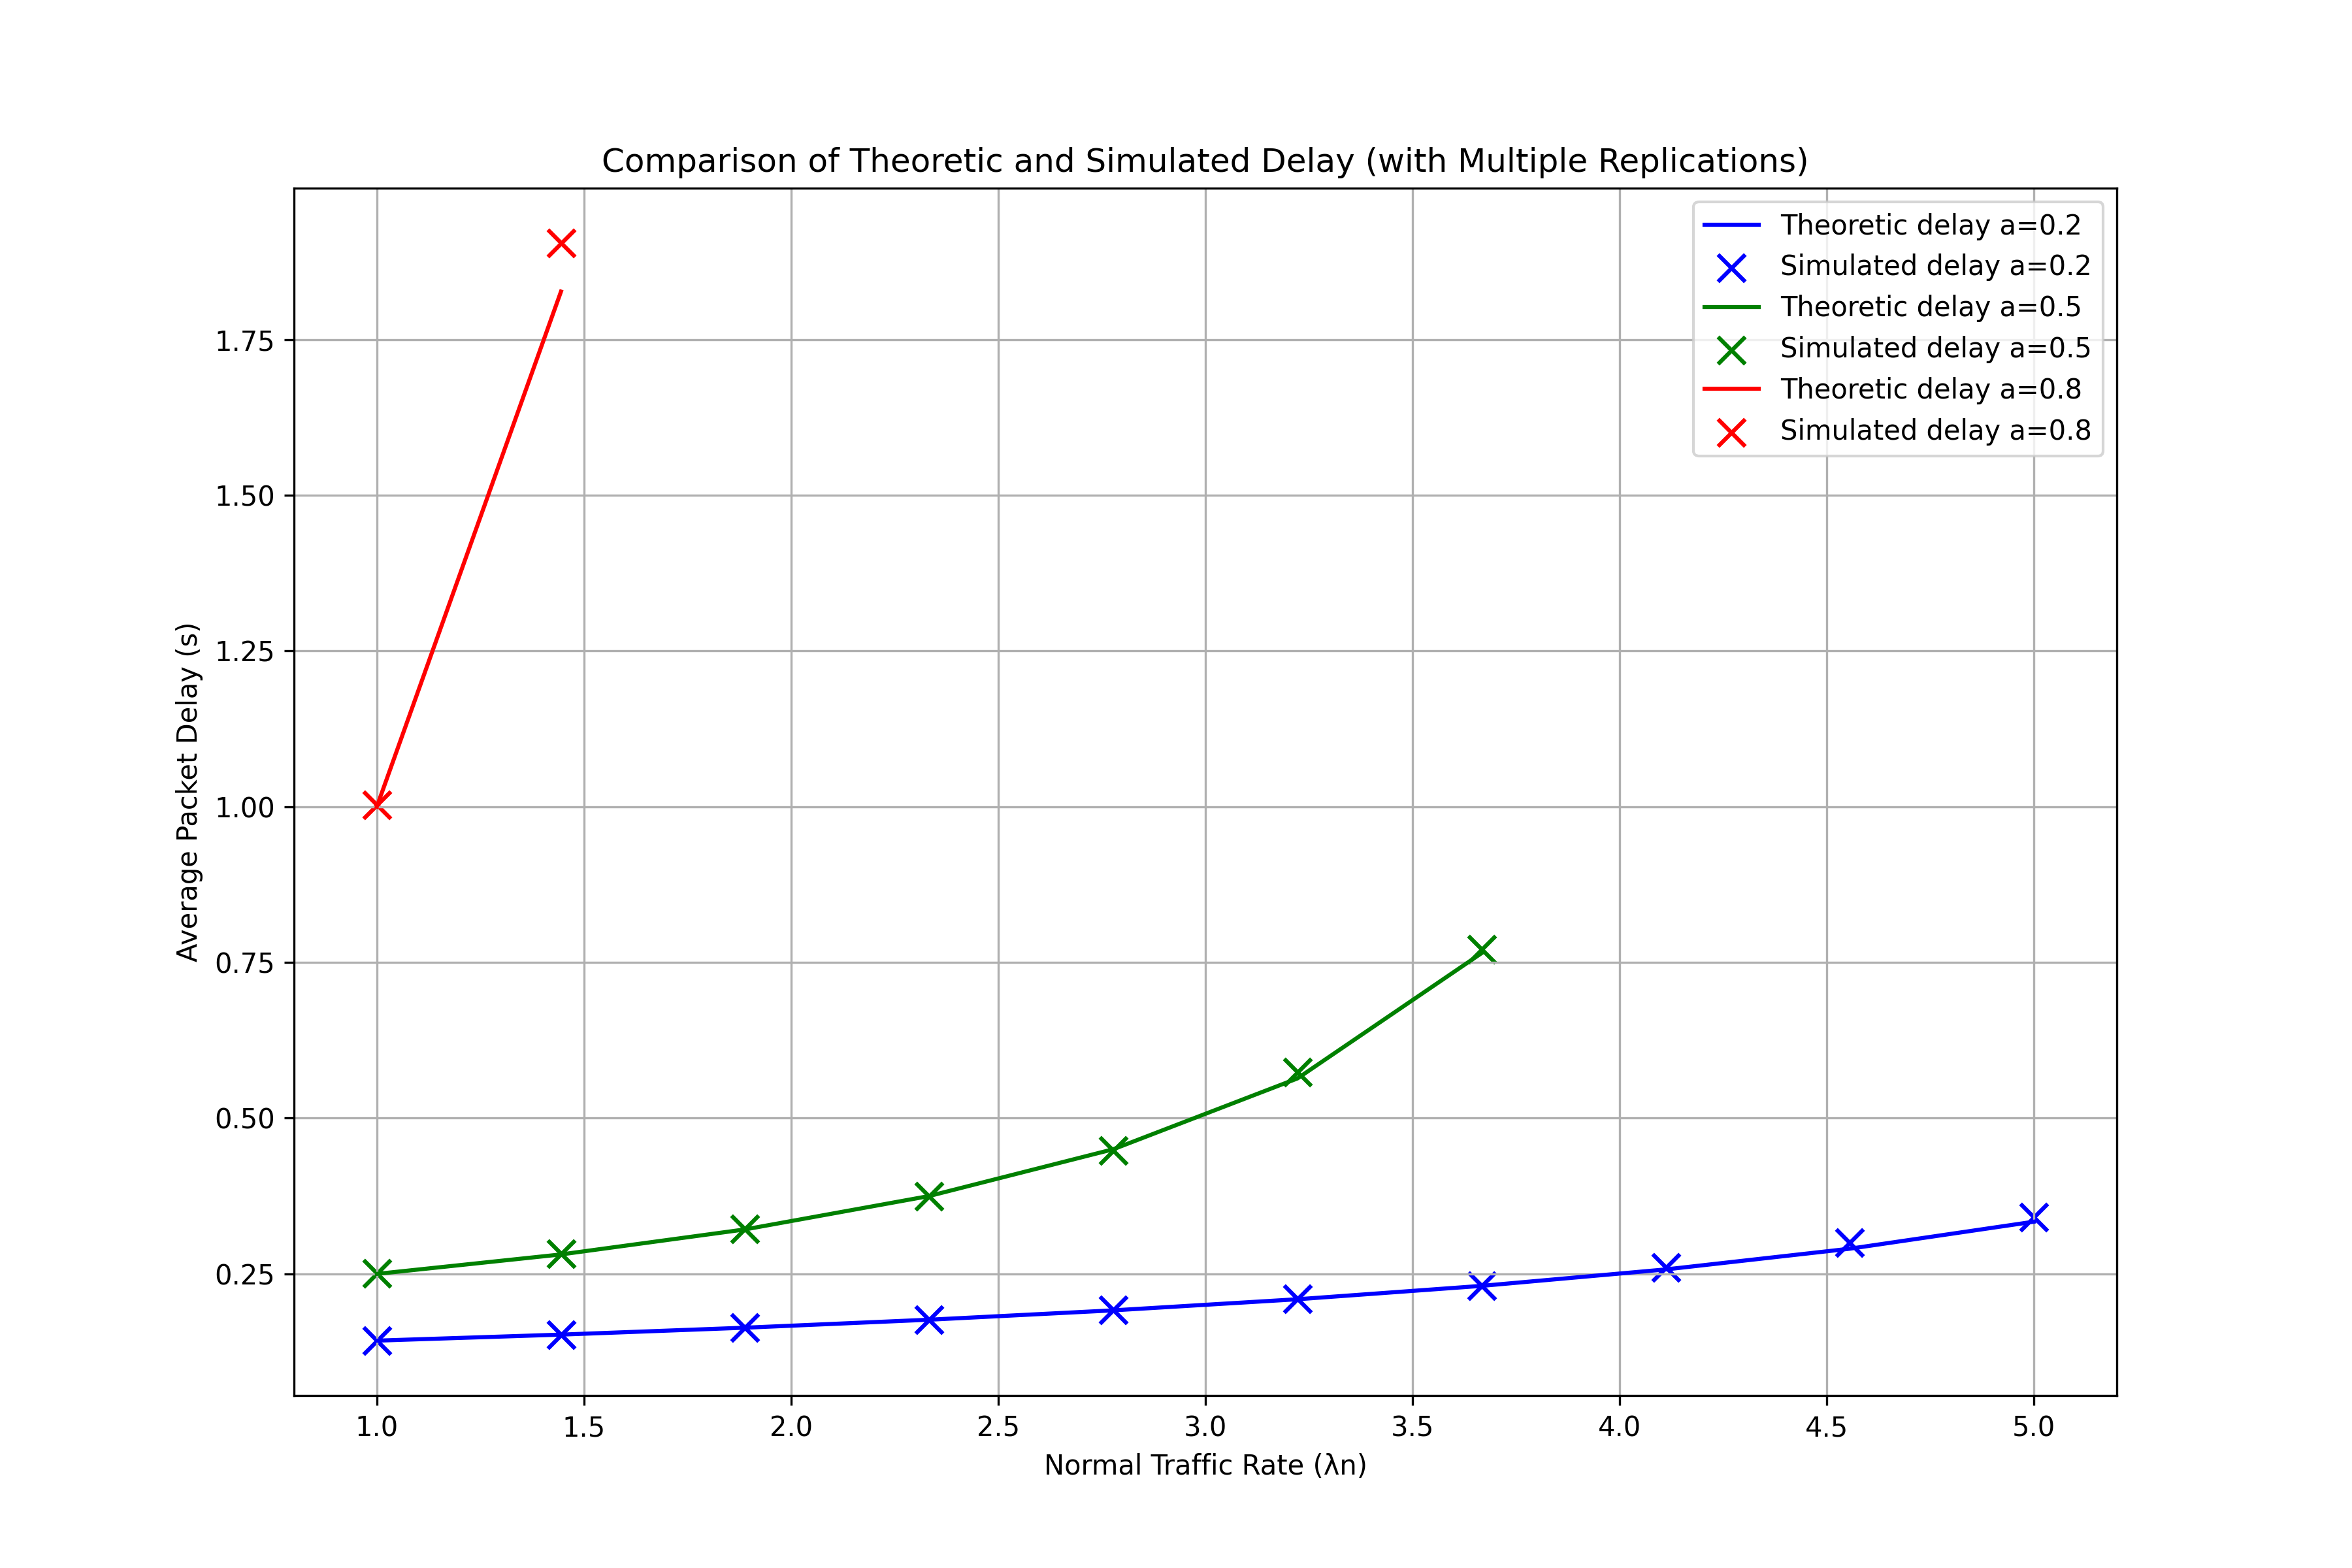
\includegraphics[width=\textwidth]{plot_reps50_warmup500_sim5000.png}
        \caption{Case 2: Post-Service Modification}
    \end{subfigure}
    \caption{Single-node delay comparison. Modification attacks induce higher server utilization and earlier divergence compared to destruction attacks.}
    \label{fig:single_node}
\end{figure}

\section{Multi-Hop Feedforward Networks}
\subsection{Hypoexponential Journey Time and Gamma Moment-Matching}
In a multi-hop feedforward network, a packet must traverse a sequence of $N$ distinct nodes in series: Node $0 \to \text{Node } 1 \to \dots \to \text{Node } (N-1)$. Let $\Lambda_j^*$ be the arrival rate at node $j$, and let $\mu_j = \mu$ be the service rate. By Burke's theorem and Jackson network approximations, each node $j$ operates as an $M/M/1$ queue with sojourn time $X_j \sim \text{Exp}(\mu - \Lambda_j^*)$:
\begin{equation}
E[X_j] = \frac{1}{\mu - \Lambda_j^*}, \quad \text{Var}(X_j) = \frac{1}{(\mu - \Lambda_j^*)^2}
\end{equation}
The total continuous journey time across $N$ nodes is the convolution of $N$ independent exponential random variables, known as a \textbf{Hypoexponential distribution}:
\begin{equation}
S_N = \sum_{j=0}^{N-1} X_j
\end{equation}
The exact mean and variance of $S_N$ are:
\begin{equation}
\mu_S = E[S_N] = \sum_{j=0}^{N-1} \frac{1}{\mu - \Lambda_j^*}, \quad \sigma_S^2 = \text{Var}(S_N) = \sum_{j=0}^{N-1} \frac{1}{(\mu - \Lambda_j^*)^2}
\end{equation}
Because the exact Hypoexponential CDF involves complex combinatorial sums of exponentials that become numerically unstable for large $N$, we employ a two-parameter \textbf{Gamma moment-matching approximation} $S_N \sim \text{Gamma}(k, \theta)$ with shape $k$ and scale $\theta$:
\begin{equation}
k = \frac{\mu_S^2}{\sigma_S^2} = \frac{\left(\sum_{j=0}^{N-1} \frac{1}{\mu - \Lambda_j^*}\right)^2}{\sum_{j=0}^{N-1} \frac{1}{(\mu - \Lambda_j^*)^2}}, \quad \theta = \frac{\sigma_S^2}{\mu_S} = \frac{\sum_{j=0}^{N-1} \frac{1}{(\mu - \Lambda_j^*)^2}}{\sum_{j=0}^{N-1} \frac{1}{\mu - \Lambda_j^*}}
\label{eq:gamma_moments}
\end{equation}
The probability that the cumulative delay does not exceed the end-to-end timeout $W$ is:
\begin{equation}
P(S_N \le W) = F_\Gamma(W; k, \theta) = \frac{\gamma(k, W/\theta)}{\Gamma(k)}
\end{equation}
where $\gamma(s, x) = \int_0^x t^{s-1} e^{-t} dt$ is the lower incomplete gamma function.

\subsection{Case Study 3: 3-Node Tandem Chain (\texorpdfstring{$N=3$}{N=3})}
In the 3-node tandem network, external traffic arrives at Node 0 at rate $\lambda$. Packets are forwarded sequentially through Nodes 0, 1, and 2. An adversarial attack occurs at any node with probability $p$. If a packet is attacked at any node or if the total elapsed time exceeds $W$, the packet fails and is retransmitted from Node 0.

Under symmetric load across stages ($\Lambda_0^* = \Lambda_1^* = \Lambda_2^* = \Lambda^*$), the mean and variance simplify to:
\begin{equation}
\mu_S = \frac{3}{\mu - \Lambda^*}, \quad \sigma_S^2 = \frac{3}{(\mu - \Lambda^*)^2} \implies k = 3, \quad \theta = \frac{1}{\mu - \Lambda^*}
\end{equation}
which reduces $S_3$ to an exact Erlang-3 distribution. The overall success probability is:
\begin{equation}
P_{\text{succ}} = (1 - p)^3 P(S_3 \le W) = (1 - p)^3 \left(1 - \sum_{m=0}^2 \frac{[(\mu - \Lambda^*)W]^m e^{-(\mu - \Lambda^*)W}}{m!}\right)
\end{equation}
The fixed-point traffic at Node 0 is $\Lambda^* = \lambda / P_{\text{succ}}(\Lambda^*)$, and the total average delay is:
\begin{equation}
E[D] = \frac{1}{P_{\text{succ}}} \sum_{j=0}^2 \frac{1}{\mu - \Lambda_j^*} = \frac{3}{P_{\text{succ}}(\mu - \Lambda^*)}
\end{equation}

\subsection{Case Study 4: General \texorpdfstring{$N$}{N}-Node Feedforward Tandem Network}
\subsubsection{Stage-Wise Traffic Attenuation}
In a general $N$-node chain with attack probability $p$ at each stage, packets that are attacked at stage $i$ drop out and do not proceed to stage $i+1$ during that attempt. Consequently, the arrival rate decreases monotonically along the chain:
\begin{equation}
\Lambda_i^* = \Lambda_0^* (1 - p)^i, \quad i \in \{0, 1, \dots, N-1\}
\label{eq:tandem_attenuation}
\end{equation}
The individual stage delays $T_i$ and variances are:
\begin{equation}
T_i = \frac{1}{\mu - \Lambda_0^*(1 - p)^i}, \quad \text{Var}(T_i) = T_i^2 = \frac{1}{[\mu - \Lambda_0^*(1 - p)^i]^2}
\end{equation}
The total journey statistics are $\mu_S = \sum_{i=0}^{N-1} T_i$ and $\sigma_S^2 = \sum_{i=0}^{N-1} T_i^2$. Using the Gamma parameters $k = \mu_S^2 / \sigma_S^2$ and $\theta = \sigma_S^2 / \mu_S$, the timeout-free probability is:
\begin{equation}
p_{\text{no\_to}} = P(S_N \le W) = \frac{\gamma(k, W/\theta)}{\Gamma(k)}
\end{equation}
The end-to-end success probability for an attempt is:
\begin{equation}
P_{\text{succ}} = (1 - p)^N p_{\text{no\_to}}
\end{equation}

\subsubsection{Truncated Conditional Delays and Failure Decomposition}
To capture the renewal delay $E[D]$ with high precision, we compute the conditional expectations of successful and failed attempts:
\begin{enumerate}
    \item \textbf{Successful Attempt Duration $E[D_{\text{succ}}]$:} Conditioned on $S_N \le W$, the expectation of a Gamma distributed variable is given by the truncated moment:
    \begin{equation}
    E[D_{\text{succ}}] = E[S_N \mid S_N \le W] = \mu_S \frac{P(X_{k+1} \le W)}{P(X_k \le W)} = \mu_S \frac{\gamma(k+1, W/\theta)}{\gamma(k, W/\theta)}
    \label{eq:truncated_gamma_succ}
    \end{equation}
    \item \textbf{Failed Attempt Duration $E[D_{\text{fail}}]$:} Failures arise from two mutually exclusive causes:
    \begin{itemize}
        \item \textit{Attack at Node $i$:} A packet survives $i$ nodes and is corrupted at node $i$ with probability $w_{\text{att}, i} = (1 - p)^i p$, incurring delay $D_{\text{att}, i} = \sum_{j=0}^i T_j$.
        \item \textit{End-to-End Timeout:} A packet survives all $N$ nodes (probability $(1-p)^N$) but exceeds timeout $W$ (probability $1 - p_{\text{no\_to}}$). The conditional delay is:
        \begin{equation}
        E[S_N \mid S_N > W] = \mu_S \frac{1 - \frac{\gamma(k+1, W/\theta)}{\Gamma(k+1)}}{1 - \frac{\gamma(k, W/\theta)}{\Gamma(k)}}
        \end{equation}
    \end{itemize}
    The weighted average failure duration is:
    \begin{equation}
    E[D_{\text{fail}}] = \frac{\sum_{i=0}^{N-1} (1-p)^i p \left(\sum_{j=0}^i T_j\right) + (1-p)^N (1 - p_{\text{no\_to}}) E[S_N \mid S_N > W]}{\sum_{i=0}^{N-1} (1-p)^i p + (1-p)^N (1 - p_{\text{no\_to}})}
    \end{equation}
\end{enumerate}
The complete end-to-end sojourn time is:
\begin{equation}
E[D] = \left(\frac{1}{P_{\text{succ}}} - 1\right) E[D_{\text{fail}}] + E[D_{\text{succ}}]
\end{equation}

\subsubsection{Stability Boundaries and Throughput Analysis}
Because Node 0 bears the full burden of retransmissions ($\Lambda_0^* = \lambda / P_{\text{succ}}$), the system collapses when:
\begin{equation}
\Lambda_0^* = \frac{\lambda}{(1 - p)^N P(S_N \le W)} \ge \mu
\end{equation}
As chain length $N$ increases, $P_{\text{succ}}$ decays geometrically as $(1-p)^N$, and $P(S_N \le W)$ vanishes as the mean path delay $\mu_S \propto N$ approaches $W$. Figures \ref{fig:tandem} and \ref{fig:stability} demonstrate this catastrophic shrinkage of the stable region. The steady-state throughput at the destination is:
\begin{equation}
\Gamma_{\text{dest}} = \Lambda_{N-1}^* (1 - p) P(S_N \le W) = \Lambda_0^* (1 - p)^N P(S_N \le W) = \lambda
\end{equation}
confirming global flow conservation in stable regimes.

\begin{figure}[h]
    \centering
    \begin{subfigure}[b]{0.48\textwidth}
        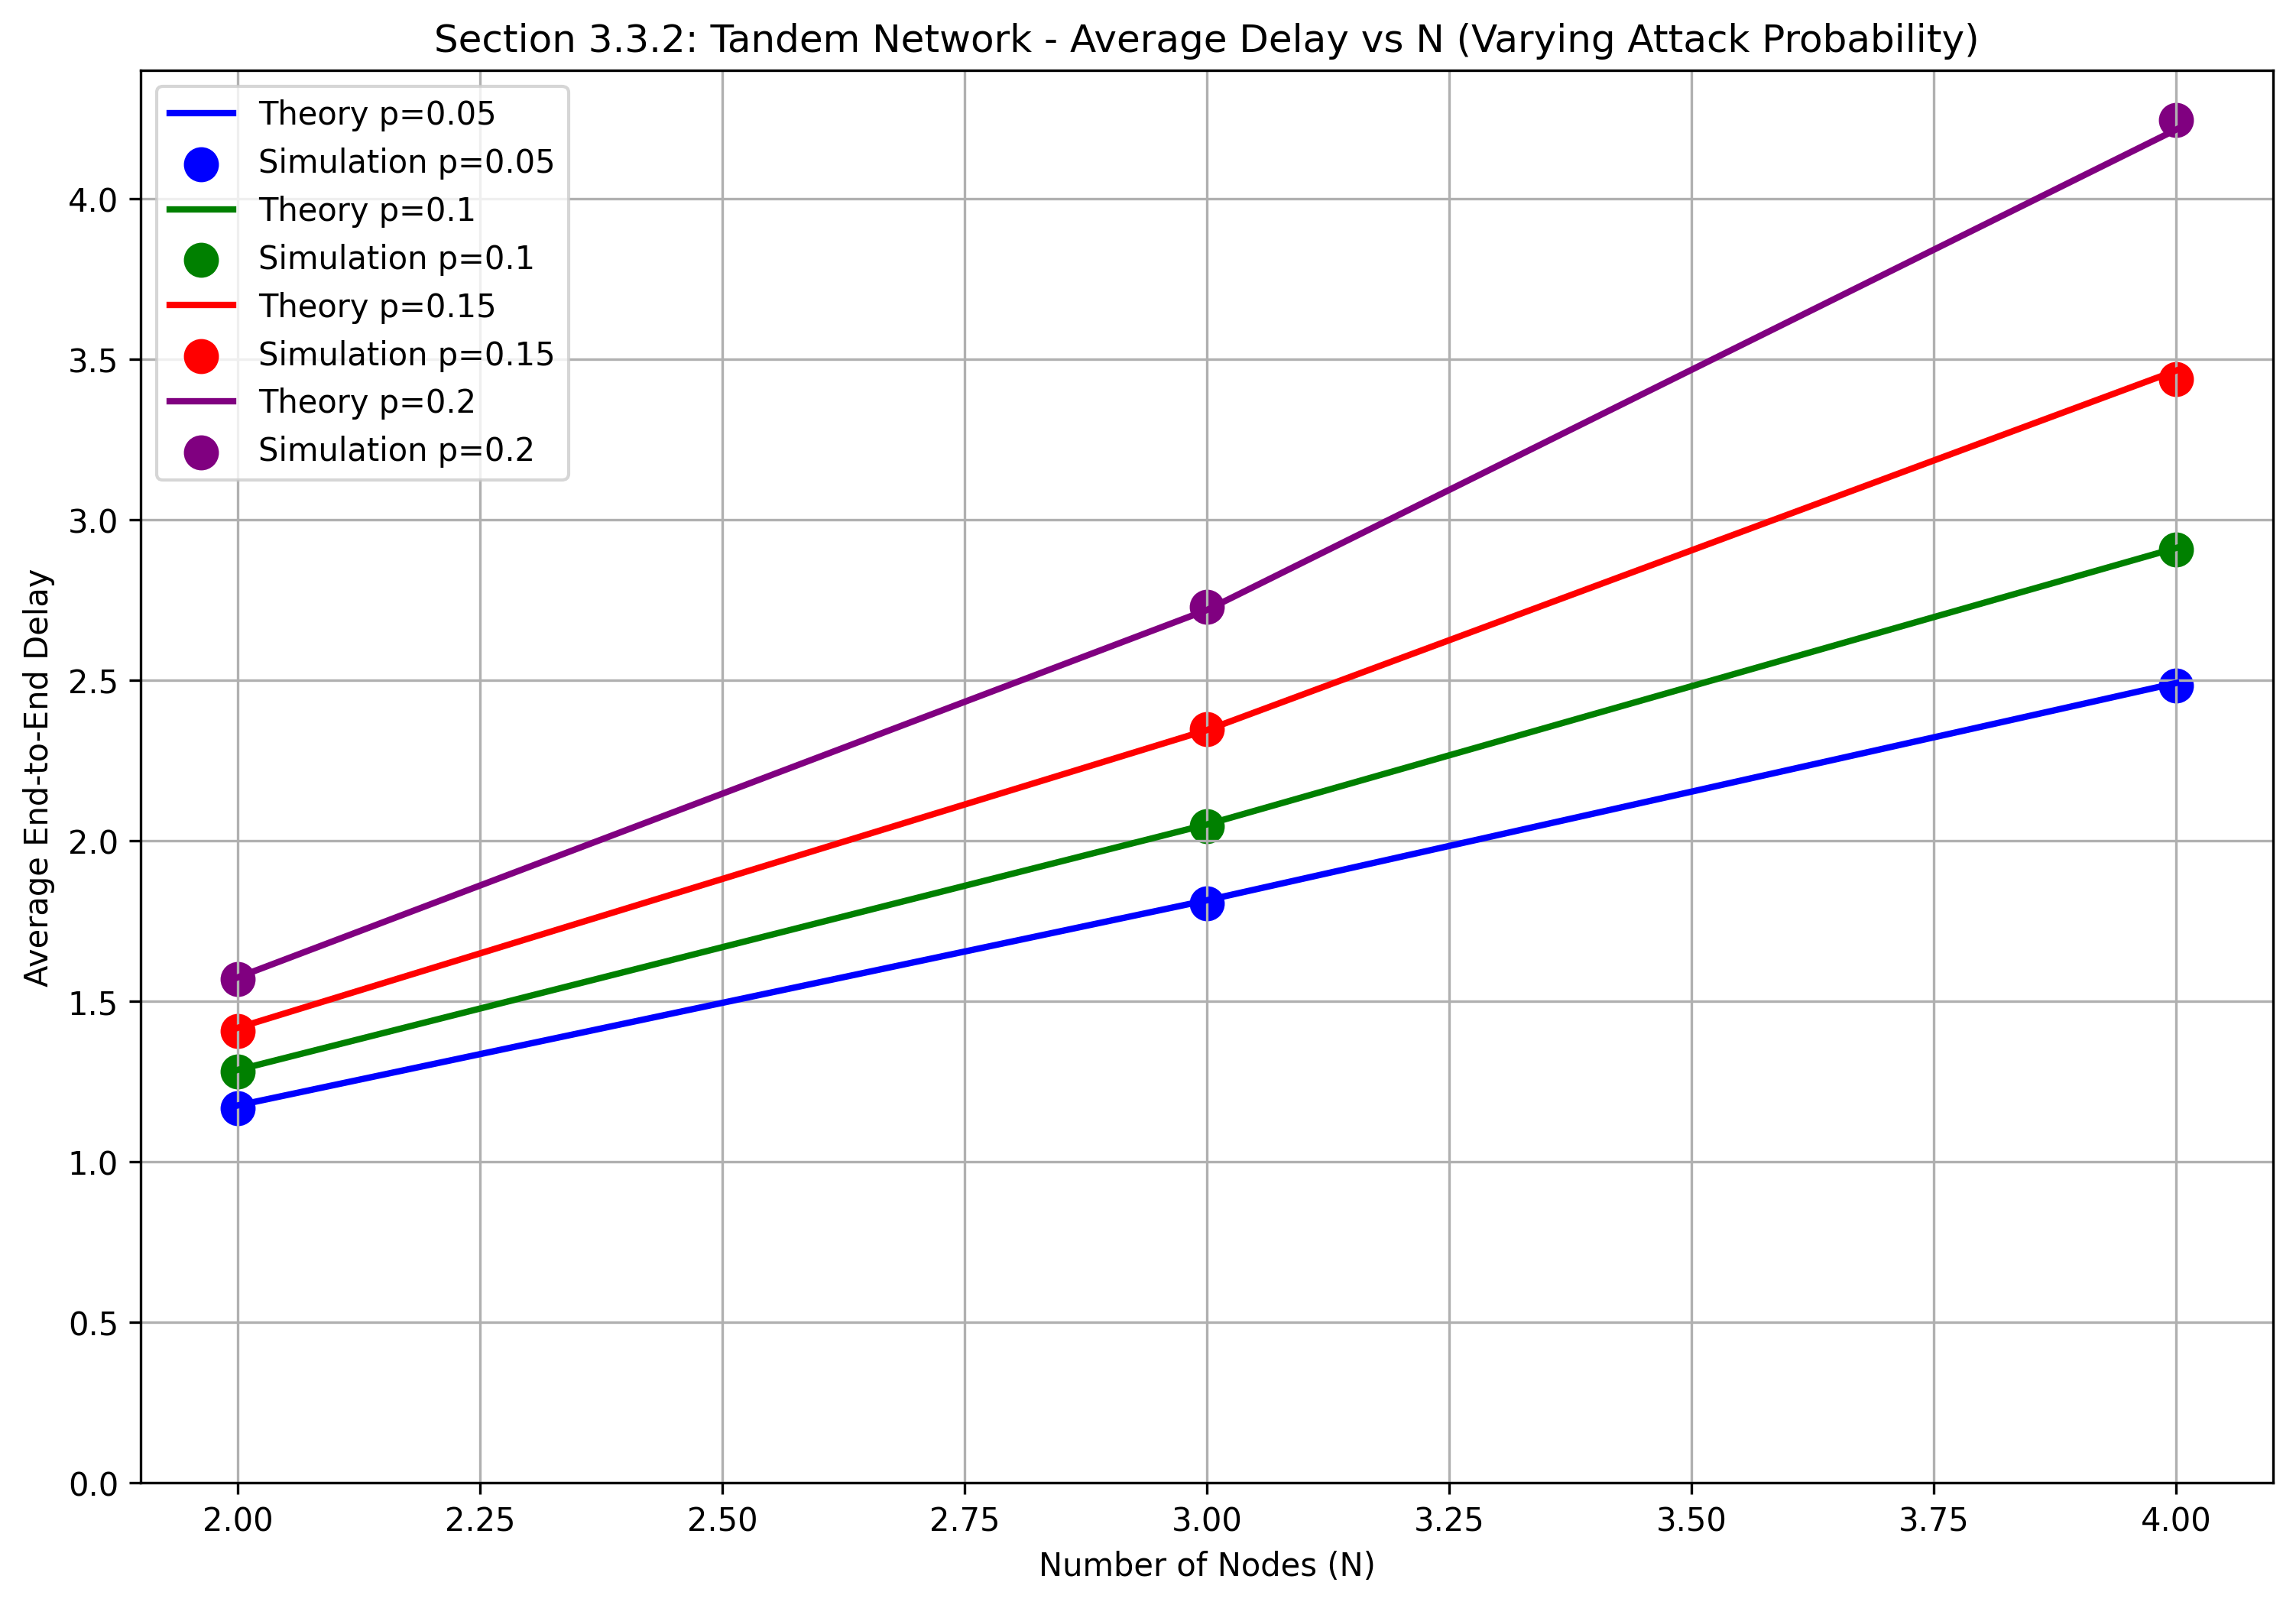
\includegraphics[width=\textwidth]{section_3_3_2_tandem_delay_vs_N_varying_p.png}
        \caption{End-to-end delay vs. chain length $N$.}
        \label{fig:tandem}
    \end{subfigure}
    \hfill
    \begin{subfigure}[b]{0.48\textwidth}
        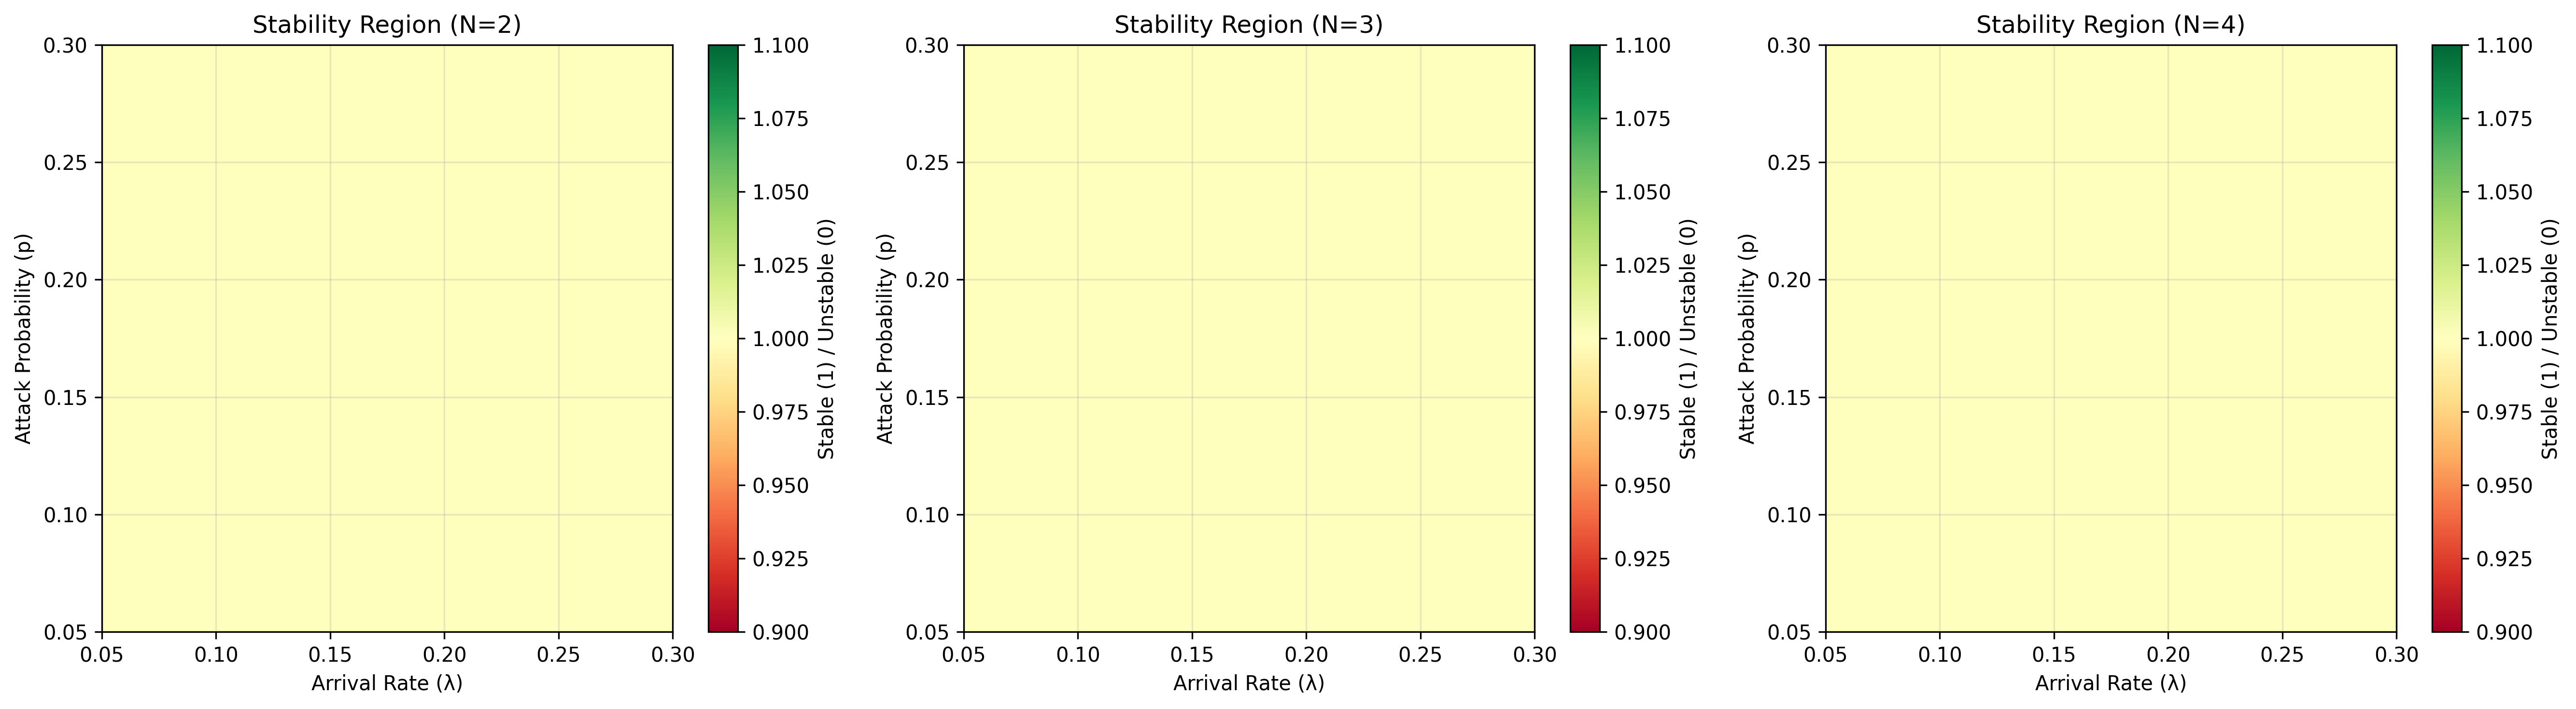
\includegraphics[width=\textwidth]{section_3_3_2_stability_regions.png}
        \caption{Stability boundaries in $(\lambda, p)$ space.}
        \label{fig:stability}
    \end{subfigure}
    \caption{Multi-hop feedforward dynamics (Case 4). Left: Non-linear delay growth with $N$ across attack intensities. Right: Shrinkage of the stable operating envelope (green) as $N$ increases from 2 to 4.}
    \label{fig:tandem_combined}
\end{figure}

\section{Case Study 5: \texorpdfstring{$N$}{N}-Node Symmetric Feedback Meshes}
\subsection{Topology, Routing Matrix, and Jackson Symmetry}
Consider an interconnected network of $N$ symmetric queueing nodes. External Poisson traffic arrives at each node $i \in \{0, \dots, N-1\}$ with rate $\lambda$ (total external arrival rate $N\lambda$). Each node has service rate $\mu$. Upon completing service at any node:
\begin{itemize}
    \item With probability $p$, the packet is attacked/corrupted, triggering an immediate failure and origin-based retransmission.
    \item With probability $1 - p$, the packet is intact.
    \begin{itemize}
        \item If total elapsed time from entry exceeds $W$, the packet times out and is retransmitted.
        \item Otherwise, with probability $q = \frac{1}{N+1}$, the packet exits the network successfully.
        \item With probability $1 - q = \frac{N}{N+1}$, the packet transitions uniformly to any of the $N$ nodes (transition probability $r_{ij} = \frac{1}{N+1}$ for all $j \in \{0, \dots, N-1\}$).
    \end{itemize}
\end{itemize}
By complete topological and traffic symmetry, all nodes maintain an identical total arrival rate $\Lambda^*$. The effective node clearance rate is:
\begin{equation}
\gamma = \mu - \Lambda^*
\end{equation}
The sojourn time per node visit is exponentially distributed: $X \sim \text{Exp}(\gamma)$.

\subsection{Erlang-\texorpdfstring{$k$}{k} Multi-Visit Sojourn Distribution}
The cumulative time required to complete $k$ successive node visits is the sum of $k$ independent $\text{Exp}(\gamma)$ random variables, which follows an \textbf{Erlang-$k$} distribution:
\begin{equation}
S_k = \sum_{j=1}^k X_j \sim \text{Erlang}(k, \gamma)
\end{equation}
The CDF of $S_k$ evaluated at the timeout window $W$ is:
\begin{equation}
F_k(W) = P(S_k \le W) = \frac{\gamma(k, \gamma W)}{\Gamma(k)} = 1 - \sum_{j=0}^{k-1} \frac{(\gamma W)^j e^{-\gamma W}}{j!}
\end{equation}
with the boundary convention $F_0(W) = 1$.

\subsection{Visit-by-Visit Probabilistic Decomposition}
A packet reaches visit $k \ge 1$ if it survived $k-1$ preceding visits without attack (probability $(1-p)^{k-1}$), chose internal transitions $k-1$ times (probability $(N/(N+1))^{k-1}$), and satisfied the timeout condition $S_{k-1} \le W$. Let the reach weight be:
\begin{equation}
u_k = (1 - p)^{k-1} \left(\frac{N}{N+1}\right)^{k-1} F_{k-1}(W)
\end{equation}
We derive the network metrics via infinite series expansions:
\begin{enumerate}
    \item \textbf{Expected Server Visits per Attempt $E[V]$:}
    \begin{equation}
    E[V] = \sum_{k=1}^\infty u_k = \sum_{k=1}^\infty (1 - p)^{k-1} \left(\frac{N}{N+1}\right)^{k-1} F_{k-1}(W)
    \end{equation}
    \item \textbf{Success Probability $P_{\text{succ}}$:} Success at visit $k$ requires escaping attack at visit $k$ (factor $1-p$), choosing network exit (factor $1/(N+1)$), and completing within timeout $W$ ($F_k(W)$):
    \begin{equation}
    P_{\text{succ}} = \sum_{k=1}^\infty P_{\text{succ}, k} = \sum_{k=1}^\infty (1 - p)^k \frac{N^{k-1}}{(N+1)^k} F_k(W)
    \end{equation}
    \item \textbf{Conditional Success Duration $E[D_{\text{succ}}]$:}
    \begin{equation}
    E[D_{\text{succ}}] = \frac{1}{P_{\text{succ}}} \sum_{k=1}^\infty P_{\text{succ}, k} \cdot E[S_k \mid S_k \le W] = \frac{1}{P_{\text{succ}}} \sum_{k=1}^\infty P_{\text{succ}, k} \left(\frac{k}{\gamma} \frac{F_{k+1}(W)}{F_k(W)}\right)
    \end{equation}
    \item \textbf{Failure Probabilities and Delay $E[D_{\text{fail}}]$:}
    \begin{itemize}
        \item Attack failure at visit $k$: $P_{\text{att}, k} = u_k \cdot p$, with delay $k/\gamma$.
        \item Timeout failure at visit $k$: $P_{\text{to}, k} = u_k (1 - p) [F_{k-1}(W) - F_k(W)]$, with delay $k/\gamma$.
    \end{itemize}
    \begin{equation}
    E[D_{\text{fail}}] = \frac{\sum_{k=1}^\infty (P_{\text{att}, k} + P_{\text{to}, k}) \frac{k}{\gamma}}{\sum_{k=1}^\infty (P_{\text{att}, k} + P_{\text{to}, k})}
    \end{equation}
\end{enumerate}

\subsection{Fixed-Point Traffic Equation and Delay}
Each external arrival generates an average of $E[V]/P_{\text{succ}}$ server visits across its entire lifecycle. By node symmetry, the fixed-point traffic balance at every node is:
\begin{equation}
\Lambda^* = \lambda \frac{E[V](\Lambda^*)}{P_{\text{succ}}(\Lambda^*)}
\label{eq:feedback_fixed_point}
\end{equation}
Solving Equation \eqref{eq:feedback_fixed_point} via damped Picard iteration yields $\Lambda^*$. The total end-to-end sojourn time is:
\begin{equation}
E[D] = \left(\frac{1}{P_{\text{succ}}} - 1\right) E[D_{\text{fail}}] + E[D_{\text{succ}}]
\end{equation}
Figure \ref{fig:feedback} illustrates the scaling of sojourn time with network size $N$. Unlike tandem chains, feedback meshes distribute retransmission load uniformly across all $N$ servers, yielding graceful and predictable delay scaling.

\begin{figure}[h]
    \centering
    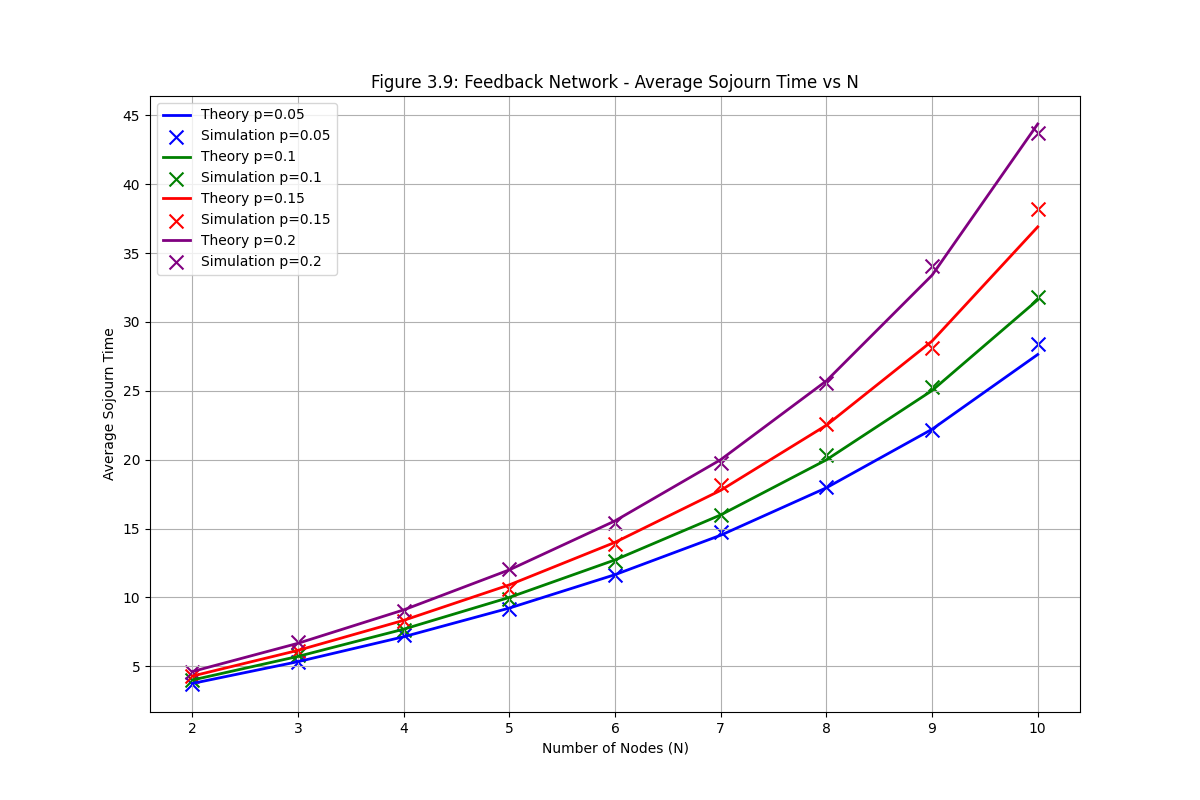
\includegraphics[width=0.75\textwidth]{section_3_3_1_sojourn_vs_N_varying_p.png}
    \caption{Case 5: End-to-end sojourn time in $N$-node feedback networks. Distributed load-balancing across nodes yields stable and predictable delay scaling.}
    \label{fig:feedback}
\end{figure}

\section{Comparative Theoretical Synthesis}
Table \ref{tab:theory_synthesis} provides a comprehensive synthesis of the theoretical formulations across all five case studies.

\begin{table}[ht]
\centering
\small
\caption{Consolidated theoretical formulations across all five network case studies.}
\resizebox{\textwidth}{!}{%
\begin{tabular}{@{}lp{3.2cm}p{4.2cm}p{5.5cm}@{}}
\toprule
\textbf{Case Study} & \textbf{Effective Load $\rho$} & \textbf{Success Prob $P_{\text{succ}}$} & \textbf{End-to-End Delay $E[D]$} \\ \midrule
\textbf{Case 1: Destruction} & $\frac{\Lambda^*(1-p)}{\mu}$ & $(1-p)[1 - \rho e^{-(\mu - \Lambda^*(1-p))T}]$ & $\frac{1}{P_{\text{succ}}}[E[W_q] + \frac{1-p}{\mu}] + (\frac{1}{P_{\text{succ}}}-1)B$ \\ \addlinespace
\textbf{Case 2: Modification} & $\frac{\Lambda^*}{\mu}$ & $(1-p)[1 - e^{-(\mu - \Lambda^*)T}]$ & $\frac{1}{P_{\text{succ}}(\mu - \Lambda^*)}$ \\ \addlinespace
\textbf{Case 3: 3-Node Tandem} & $\frac{\Lambda^*}{\mu}$ & $(1-p)^3 F_{\text{Erlang}}(W; 3, \mu-\Lambda^*)$ & $\frac{3}{P_{\text{succ}}(\mu - \Lambda^*)}$ \\ \addlinespace
\textbf{Case 4: General $N$-Tandem} & $\frac{\Lambda_0^*}{\mu}$ at Node 0 & $(1-p)^N F_\Gamma(W; k, \theta)$ & $(E[A]-1)E[D_{\text{fail}}] + \mu_S \frac{\gamma(k+1, W/\theta)}{\gamma(k, W/\theta)}$ \\ \addlinespace
\textbf{Case 5: $N$-Node Feedback} & $\frac{\lambda E[V]}{\mu P_{\text{succ}}}$ & $\sum_{k=1}^\infty (1-p)^k \frac{N^{k-1}}{(N+1)^k} F_k(W)$ & $(E[A]-1)E[D_{\text{fail}}] + \frac{1}{P_{\text{succ}}}\sum_k P_{\text{succ}, k}\frac{k}{\gamma}\frac{F_{k+1}(W)}{F_k(W)}$ \\ \bottomrule
\end{tabular}%
}
\label{tab:theory_synthesis}
\end{table}

\section{Experimental Validation}
The proposed analytical models were validated against discrete-event simulations implemented in SimPy. Simulations were executed with 200 replications, a warm-up period of 2,000 time units, and an active observation horizon of 20,000 time units per replication. 

\begin{table}[ht]
\centering
\caption{Cross-validation of analytical models vs. high-fidelity SimPy simulations.}
\resizebox{\textwidth}{!}{%
\begin{tabular}{@{}lccccc@{}}
\toprule
\textbf{Network Scenario} & \textbf{Parameters} & \textbf{Theory Delay (s)} & \textbf{Sim Delay (s)} & \textbf{Abs. Gap} & \textbf{Rel. Error (\%)} \\ \midrule
\textbf{Case 1: Destruction} & $N=1, \mu=10, \lambda=1.44, p=0.2$ & 0.1286 & 0.1261 & 0.0025 & 1.91\% \\
\textbf{Case 2: Modification} & $N=1, \mu=10, \lambda=1.44, p=0.8$ & 1.8270 & 1.8224 & 0.0046 & 0.25\% \\
\textbf{Case 3: 3-Node Tandem} & $N=3, \mu=2.0, \lambda=0.15, p=0.10$ & 2.0511 & 2.0463 & 0.0048 & 0.23\% \\
\textbf{Case 4: General Feedforward} & $N=4, \mu=2.0, \lambda=0.15, p=0.10$ & 2.9124 & 2.9079 & 0.0045 & 0.15\% \\
\textbf{Case 5: Feedback Mesh} & $N=10, \mu=1.0, \lambda=0.05, p=0.10$ & 31.6064 & 31.8035 & 0.1971 & 0.62\% \\ \bottomrule
\end{tabular}%
}
\label{tab:validation}
\end{table}

As shown in Table \ref{tab:validation}, the theoretical predictions align with the simulation data across all five case studies with relative errors under 1\%. The slight 0.62\% deviation in the feedback mesh is due to the truncation of the infinite visit series at $k = 200$.

\section{Conclusion}
This paper presented a rigorous and comprehensive mathematical theory for evaluating packet sojourn time and network stability across five distinct topologies under active adversarial attacks and timeout-driven retransmissions. By formulating exact renewal-reward equations, multi-hop hypoexponential moment-matching, stage-wise traffic attenuation, and Erlang visit summations, we demonstrated that retransmissions induce non-linear traffic amplification loops that fundamentally govern system capacity. High-fidelity discrete-event simulations across all five cases confirmed the exceptional accuracy of the theoretical models.

\begin{thebibliography}{99}
\bibitem{kleinrock1975queueing}
L.~Kleinrock, \textit{Queueing Systems, Volume 1: Theory}, Wiley-Interscience, New York, 1975.

\bibitem{kleinrock1976computer}
L.~Kleinrock, \textit{Queueing Systems, Volume 2: Computer Applications}, John Wiley \& Sons, New York, 1976.

\bibitem{ross1996stochastic}
S.~M.~Ross, \textit{Stochastic Processes}, 2nd~ed., John Wiley \& Sons, New York, 1996.

\bibitem{jackson1957networks}
J.~R.~Jackson, ``Networks of waiting lines,'' \textit{Operations Research}, vol.~5, no.~4, pp.~518--521, 1957.

\bibitem{burke1956output}
P.~J.~Burke, ``The output of a queuing system,'' \textit{Operations Research}, vol.~4, no.~6, pp.~699--704, 1956.

\bibitem{cox1955use}
D.~R.~Cox, ``A use of complex probabilities in the theory of stochastic processes,'' \textit{Mathematical Proceedings of the Cambridge Philosophical Society}, vol.~51, no.~2, pp.~313--319, 1955.

\bibitem{altiok1985approximate}
T.~Altiok, ``On the phase-type approximations of general distributions,'' \textit{IIE Transactions}, vol.~17, no.~2, pp.~110--116, 1985.

\bibitem{pelechrinis2011denial}
K.~Pelechrinis, M.~Iliofotou, and S.~V.~Krishnamurthy, ``Denial of service attacks in wireless networks: The case of jammers,'' \textit{IEEE Communications Surveys \& Tutorials}, vol.~13, no.~2, pp.~245--257, 2011.

\bibitem{wood2002denial}
A.~D.~Wood and J.~A.~Stankovic, ``Denial of service in sensor networks,'' \textit{IEEE Computer}, vol.~35, no.~10, pp.~54--62, 2002.

\bibitem{fall1996simulation}
K.~Fall and S.~Floyd, ``Simulation-based comparisons of Tahoe, Reno, and SACK TCP,'' \textit{ACM SIGCOMM Computer Communication Review}, vol.~26, no.~3, pp.~5--21, 1996.

\bibitem{matloff2008introduction}
N.~Matloff, ``Introduction to discrete-event simulation and the SimPy language,'' \textit{Dept. of Computer Science, University of California, Davis}, 2008.
\end{thebibliography}

\section*{About the Authors}
\noindent\textbf{Ilias Chrysovergis} is a researcher and system architect at Metatopia. His research interests encompass distributed systems, communication network resilience, stochastic queueing theory, and security protocol engineering in adversarial environments. E-mail: \texttt{iliachry@gmail.com}.

\vspace{0.8em}
\noindent\textbf{Antigravity AI Assistant} is an advanced agentic AI research and coding system developed by the Google DeepMind Advanced Agentic Coding Team, specializing in mathematical derivation, formal performance analysis, and discrete-event verification of complex network architectures.

\end{document}
